\sect{System Architecture}
\label{subsec:system-architecture}

\subsect{Tree Parameters}
\label{subsec:tree-parameters}

\subsubsect{Relations of Parameters}

In order to reap the full benefit of the tree data structure, an informed choice
of parameters must be made that takes consideration of the expected workload and
usage of scarce memory resources.

The tree's branching factor $m$ defines the maximum number of children that each
node can have (as well as its minimum, which is $m/2$). A level $k$ down the
tree from the root will contain $m^k$ nodes. Thus, a full tree of height $h$
will contain $\sum_{k=1}^h m^k = \frac{1-m^h}{1-m}$ nodes.

The ratio of leaf nodes to internal nodes is given by:
$$
	\frac{m^{h-1}}{\pfrac{1-m^{h-1}}{1-m}}
	= \frac{m^{h-1}(1-m)}{1-m^{h-1}}
	= \frac{m^{h-1}-m^{h}}{1-m^{h-1}}
	% = \frac{m^h-m^{h+1}}{m-m^h}
	% = \frac{m^h(1-m)}{m^h(m^{1-h} - 1)}
	= \frac{1-m}{m^{1-h} - 1}
$$

As $h$ increases, this rapidly converges to $m-1$ as shown in
\autoref{fig:inner-to-height}.

\begin{figure}[h]
	\centering
	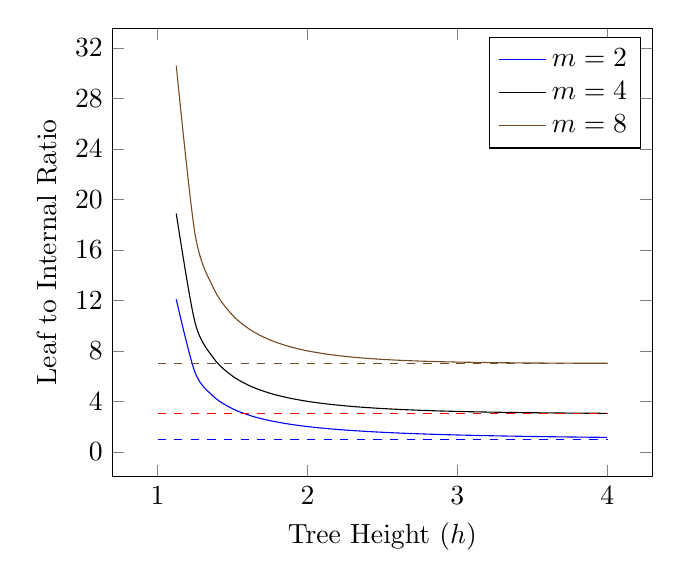
\begin{tikzpicture}
	\begin{axis}
		[
			xlabel={Tree Height ($h$)},
			ylabel={Leaf to Internal Ratio},
			xtick distance=1,
			ytick distance=4,
			domain=1:4,
			smooth
		]
		\pgfplotsinvokeforeach{2,4,8} {
			\addplot+[cycle list name=color list, mark=none]
				{(1-#1) / (#1^(1-x) - 1)};
			\addlegendentry{$m=#1$}
		}
		\pgfplotsset{cycle list shift=-3};
		\pgfplotsinvokeforeach{2,4,8} {
			\addplot+[cycle list name=color list, mark=none, dashed] {#1-1};
		}
	\end{axis}
\end{tikzpicture}

	\caption{Leaf to Inner Node Ratio vs Height}
	\label{fig:inner-to-height}
\end{figure}

As the height of a tree grows, the portion of overall memory that is used for
leaves decreases, converging to $1-\frac{1}{m}$ as shown in
\autoref{fig:memory-to-height}. Higher branching factors spend less of their
total memory on internal nodes, which only store traversal data.

\begin{figure}[H]
	\centering
	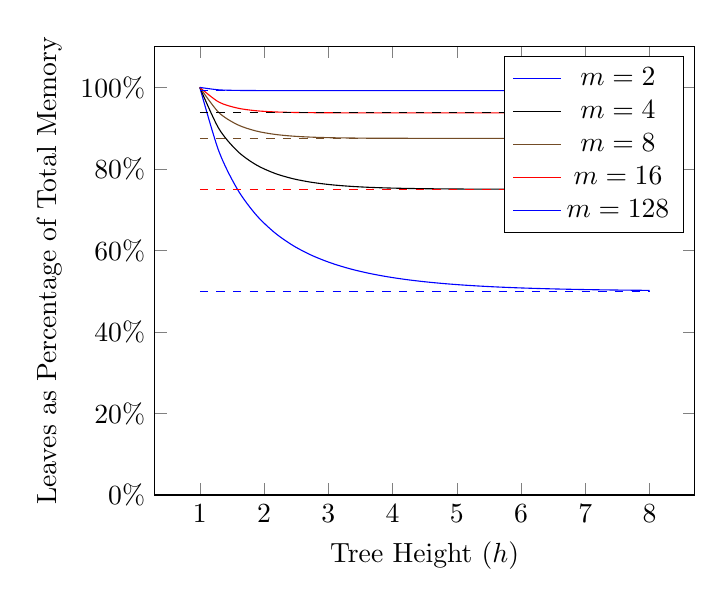
\begin{tikzpicture}
	\begin{axis}
		[
			xlabel={Tree Height ($h$)},
			ylabel={Leaves as Percentage of Total Memory},
			xtick distance=1,
			yticklabel={%
				\pgfmathparse{\tick*100}%
				\pgfmathprintnumber{\pgfmathresult}%
				\%%
			},
			domain=1:8,
			ymin=0,
			smooth
		]
		\pgfplotsinvokeforeach{2,4,8,16,128} {
			\addplot+[cycle list name=color list, mark=none]
				{#1^(x-1) / ((1-#1^x)/(1-#1))};
			\addlegendentry{$m=#1$}
		}
		\pgfplotsset{cycle list shift=-5}
		\pgfplotsinvokeforeach{2,4,8,16,128} {
			\addplot+[cycle list name=color list, mark=none, dashed]
				{1-(1/#1)};
		}
	\end{axis}
\end{tikzpicture}

	\caption{Leaves as Percentage of Total Memory vs Height}
	\label{fig:memory-to-height}
\end{figure}

A tree containing $N$ nodes will have the height shown below.

\begin{align*}
	N &= \frac{1-m^h}{1-m} \\
	N (1-m) &= 1-m^h \\
	N (1-m) - 1 &= -m^h \\
	1 - N (1-m) &= m^h \\
	\log_m\left(1 - N (1-m)\right) &= h
\end{align*}

As $N$ grows, this relation can be approximated as $h \approx 1 + \log_m(N)$,
which is equivalent to  $m^{h-1} \approx N$. Because $m^{h-1}$ is the number of
leaf nodes, this expression approximates the total count of nodes as the number
of leaf nodes. As follows from previous derivations and shown in
\autoref{fig:nodes-to-height}, this approximation is more accurate for larger $m$
where there are more leaves per inner node.

\begin{figure}[H]
	\centering
	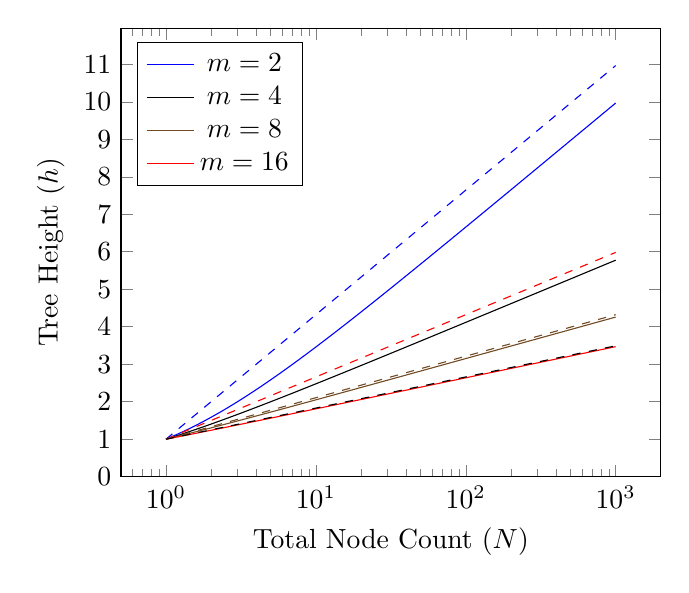
\begin{tikzpicture}
	\begin{axis}
		[
			xlabel={Total Node Count ($N$)},
			ylabel={Tree Height ($h$)},
			domain=1:1000,
			xmode=log,
			ytick distance=1,
			legend pos=north west,
			smooth
		]
		\pgfplotsinvokeforeach{2,4,8,16} {
			\addplot+[cycle list name=color list, mark=none]
				{ln(1 - x*(1-#1)) / ln(#1)};
			\addlegendentry{$m=#1$}
		}
		\pgfplotsset{cycle list shift=-4}
		\pgfplotsinvokeforeach{2,4,8,16} {
			\addplot+[cycle list name=color list, mark=none, dashed]
				{1+ln(x)/ln(#1)};
		}
	\end{axis}
\end{tikzpicture}

	\caption{Height vs Node Count}
	\label{fig:nodes-to-height}
\end{figure}


\subsubsect{Choosing Parameters}

The optimal choice of tree parameters will likely be different between FPGA and
CPU implementations due to optimizations that HLS can make to source code that
are infeasible or impossible on a CPU.

When checking all of a node's keys in order to find a specific key, a CPU must
evaluate each key one at a time. The can be accelerated with binary search so
that it can be performed in $O(\log_2 m)$, but for common $m$ values the
overhead of binary search erodes most gains compared over a simple linear
search. However, on an FPGA all keys can be evaluated \emph{simultaneously},
i.e. $O(1)$, and in fact this is Vitis' default behavior when translating
\texttt{for} loops with a sufficiently low, constant iteration count into
hardware. Larger loops can also be forced to behave this was using pre-processor
directives.

% TODO: mention upper bound from O(m) insertion


\subsect{Concurrency}
\label{subsec:concurrency}

Our tree's design is based on that of \citeauthor{base} in \citetitle{base}.
Their design uses a CPU cluster with an RDMA interconnect. The design follows
the Network-Attached-Memory (NAM) architecture, where some nodes are dedicated
to computation while others are dedicated to storage
\autocite{base,binnig-vldb-2016}.

To support concurrent access, their design uses optimistic lock coupling rather
than traditional lock coupling. This strategy does not protect areas from
concurrent access, but simply identifies when data has been changed. If two
writers begin modifying the same data, the one who writes back to main memory
second will see that its version number is not what was expected, and attempt to
restart its operation using this new data.

A key advantage of this strategy is reducing cache misses on multi-core CPUs.
Frequently changing lock bits in main memory forces constant cache
invalidations, many of which are unnecessary in read-dominated workloads
\autocite{leis-damon-2016}. On an FPGA, we have the freedom to design our own
caching protocol rather than simply mimicking the general purpose caching
protocols that are fixed in the silicon of CPUs. Thus, this problem could be
negated by managing lock bits differently from other memory.
%
For example, if each reader and writer module has its own cache, it could be set
up such that changes to lock bits only trigger invalidations for writers, since
readers never look at lock bits. As noted by \citeauthor{binnig-vldb-2016},
DBMSs function best with full control over memory management
\autocite{binnig-vldb-2016}, and this level of control is simply impossible on a
CPU.


\subsect{Memory Layout}
\label{subsec:memory-layout}

Though FPGAs still have a memory hierarchy as shown in
\autoref{fig:memory-hierarchy}, it functions differently to that of a CPU. The
datasheet for the U280 lists counts of these elements rather than a raw size in
bytes because individual modules will have dedicated connections to separate BRAM
elements rather than sharing a single cache.

\begin{figure}[H]
	\centering
	\begin{subfigure}{16em}
	\centering
	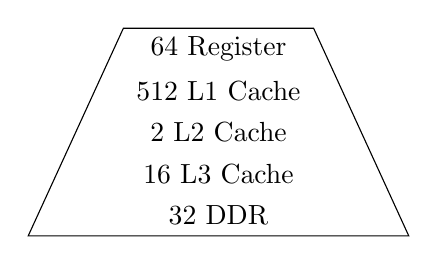
\begin{tikzpicture}[x=2.75em,y=1.5em]
		\draw (1.25, -0.5) -- ++(-2.5, 0)
			-- (-2.5, -5.5) -- ++(5, 0)
			-- cycle;
		\node at (0, -1) {$\SI{64}{\byte}$ Register};
		\node at (0, -2) {$\SI{512}{\kibi\byte}$ L1 Cache};
		\node at (0, -3) {$\SI{2}{\mebi\byte}$ L2 Cache};
		\node at (0, -4) {$\SI{16}{\mebi\byte}$ L3 Cache};
		\node at (0, -5) {$\SI{32}{\giga\byte}$ DDR};
	\end{tikzpicture}
	\caption{CPU Memory Heirarchy}
\end{subfigure}
\begin{subfigure}{16em}
	\centering
	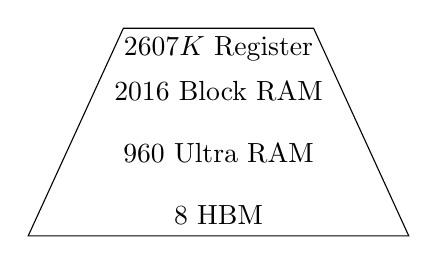
\begin{tikzpicture}[x=2.75em,y=1.5em]
		\draw (1.25, -0.5) -- ++(-2.5, 0)
			-- (-2.5, -5.5) -- ++(5, 0)
			-- cycle;
		\node at (0, -1) {$\SI{2607}{K}$ Register};
		\node at (0, -2) {$\num{2016}$ Block RAM};
		\node at (0, -3.5) {$\num{960}$ Ultra RAM};
		\node at (0, -5) {$\SI{8}{\giga\byte}$ HBM};
	\end{tikzpicture}
	\caption{FPGA Memory Heirarchy}
\end{subfigure}


% Type     | Count | Size   |
% ---------+-------+--------+
% Register | 2607K |        |
% BRAM     | 2016  | 36K    |
% URAM     |  960  | 288 Kb |
%
% Source DS963, UG440, AM007

	\caption{Memory Hierarchy Comparison}
	\label{fig:memory-hierarchy}
\end{figure}

Even without the considerations of caching that would arise on CPU-based
systems, memory access patterns can still have significant performance impacts.
The XCU280 FPGA integrates $\SI{8}{\giga\byte}$ of on-chip High-Bandwidth Memory
(HBM) with a theoretical maximum bandwidth of $\SI{460}{\giga\byte\per\second}$
\autocite{u280}, but this is contingent on spreading out the accesses across all
available channels \autocite{holzinger-ipdpsw-2021}.
% 
Though using HLS prevents some of the lower-level HBM access optimizations
proposed by \citeauthor{holzinger-ipdpsw-2021} \autocite{holzinger-ipdpsw-2021},
there remains the coarse-grained option to choose between HBM and traditional
DDR. For non-parallel access patterns, it is often faster to use DDR memory, as
its lower latency offers superior performance for single-threaded accesses.

Beyond memory technologies, it is still possible to reap some benefits by
controlling memory access patterns. Because the manner that the abstract tree is
accessed is dictated by \citeauthor{b-link}'s original algorithm, the best way
to optimize memory accesses is to consider how best to lay out the tree in
memory.

Because each level of the tree has a known maximum width for a given height and
branching factor $m$, each level can be assigned a fixed segment of memory. The
starts, ends, and widths of these segments are stored in lookup tables. The tree
is stored ``bottom to top'' in order of memory addresses.

The first node is created as the far left leaf on the bottom of the tree rather
than at the node where the root of a full tree would reside. This is because in
split operations, the newly created nodes are parent and sibling, not children.
Leaving the first node at this address means that it never needs to be moved and
thus any pointers to it from higher levels never need to be updated. The
location of the root node is a shared variable accessible by all threads.

% When inserting an entry into a node, a new node is allocated only if the node is
% already full. This a pointer to this new sibling is inserted into the original
% node's parent, which in a worse case scenario can lead to a cascade of splitting
% nodes all the way up the tree.

A single node can hold $d_1=m$ entries, thus a tree of height 1 can hold $m$
entries. A tree of height 2 can hold $d_2 = (1)m +
(d_1-1)\left\lfloor{m/2}\right\rfloor = (d_1+1)\left\lfloor{m/2}\right\rfloor$
entries, as each entry from the last level of the tree corresponds to one node
at this level of the tree. Insertions can occur until a node is full, which in
the extreme case leaves all other nodes as half full.
%
This recursive expression can be generalized to any tree height, yielding:

{\ssp$$
	d_h = \begin{cases}
		m & h = 1 \\
		(d_{h-1}+1)\left\lfloor{m/2}\right\rfloor & h > 1 \\
	\end{cases}
$$}

Recall that as shown in \autoref{fig:nodes-to-height}, the memory required for a
full tree increases exponentially with each level added. When allocating large
trees, the underfull levels resulting from the above strategy yield substantial
memory savings. If a full tree were allocated, the exponential increases in size
of the lower levels of a tree may result in allocating far more memory than is
need for a given application, which can result in allocation failures.
%
For example on an $m=8$ tree, 9 levels are required to store 611,668 entries,
but storing the 611,669th entry requires 10 levels. If a full tree were
allocated, this would balloon its size by a factor of $m$ from 19 million nodes
to 153 million nodes in order to store a single extra entry.

A Python script has been created to automate the process of deriving the correct
level widths and memory size for a given $m$ value and maximum entry count.
While it is possible to store more than the given entry maximum, it is not
successful insertion is not guaranteed.


\subsect{FPGA Implementation}
\label{subsec:fpga-implementation}

\begin{figure}[H]
	\centering
	\begin{tikzpicture}[
	node distance = 0.5cm and 1cm,
	every node/.style={align=center, execute at begin node={\baselineskip=12pt}},
	mem/.style={draw, text width=4em},
	mod/.style={draw, text width=4em},
]
	% Modules
	\node[mem] (data-mem) {Data Memory};
	\node[mem, below=of data-mem] (req-mem) {Request Memory};
	\node[mem, below=of req-mem] (resp-mem) {Response Memory};
	\node[mod, right=of req-mem] (decoder) {Request Decoder};
	\node[mod, right=of resp-mem] (encoder) {Response Encoder};
	\node[mod, right=of decoder] (search) {Search Module};
	\node[mod, right=of encoder] (insert) {Insert Module};
	% Boundaries
	\draw[dashed] ($(data-mem.north west)+(-0.3,0.3)$)
		rectangle ($(resp-mem.south east)+(0.3,-0.3)$);
	\node[above=12pt of data-mem.north] {Shared with Host};
	% Connections
	\draw[->] (req-mem) -- (decoder);
	\draw[<-] (resp-mem) -- (encoder);
	\draw[->] ($(decoder.east)+(0,0.1)$) -- ($(search.west)+(0,0.1)$);
	\draw[->] ($(decoder.east)+(0,-0.1)$) -- ++(1em, 0)
		-- ($(insert.west)+(-1em,0.1)$) -- ++(1em, 0);
	\draw[<-] ($(encoder.east)+(0,0.1)$) -- ++(1em, 0)
		-- ($(search.west)+(-1em,-0.1)$) -- ++(1em, 0);
	\draw[<-] ($(encoder.east)+(0,-0.1)$) -- ($(insert.west)+(0,-0.1)$);
	\draw[->] ($(data-mem.east)+(0,-0.1)$) -| ($(search.east)+(0.4,0.0)$) -- ++(-0.4, 0);
	\draw[<->] ($(data-mem.east)+(0,0.1)$) -| ($(insert.east)+(0.6,0.0)$) -- ++(-0.6, 0);
\end{tikzpicture}

	\caption{Architecture of HLS Kernel}
	\label{fig:hls-arch}
\end{figure}

The FPGA's HLS implementation wraps a C implementation of the B-Link tree that
uses purely statically allocated memory. I/O between the host CPU system and the
FPGA is performed over PCIe using shared memory buffers. Separate buffers are
used for instructions and data memory, as this both simplifies access and gives
Vitis more flexibility to parallelize access to these buffers in order to
maximize memory bandwidth utility.

The compute kernel itself consists of four modules as shown in
\autoref{fig:hls-arch}; two handle I/O encoding/decoding and two handle tree
operations. Requests and responses are similar in structure to CPU instructions;
a short opcode at the front delineates the operation and the remaining bits are
instruction specific, though care has been taken to align identical fields
shared between instructions so that they appear at the same offset; for example,
both search and insert requests require a key as an argument. Operations other
than \texttt{NOP} return a status code indicating whether the operation
succeeded and the cause of its failure if applicable.

Though each search \& insert module can only handle one request at a time,
multiple copies of the kernel can be instantiated on the same FPGA, each of
which share the same host memory but with separate request/response buffers,
allowing for an analog to CPU multithreading.
